\documentclass[main.tex]{subfiles}
\begin{document}

\subsection{Azure Quantum Basics} 

    The first step in using Azure Quantum is to create a \href{https://portal.azure.com/#create/Microsoft.AzureQuantum}{Quantum Workspace} shown in Figure \ref{fig:quantumWorkspace}. Once created the user can select from a set of quantum hardware providers including: IonQ, Quantinuum, and Microsoft Quantum-Inspired Optimization (QIO). IonQ provides the option to use either quantum simulation \texttt{ionq.simulator} with access to 29  simulated qubits or quantum processing unit hardware \texttt{ionq.qpu} with 11 IonQ trapped-ion qubits. The Q\# language is used to define the users quantum algorithm and is executed in Jupyter notebook cells running in the Quantum Workspace.\\
    
    \begin{figure}
        \centering
        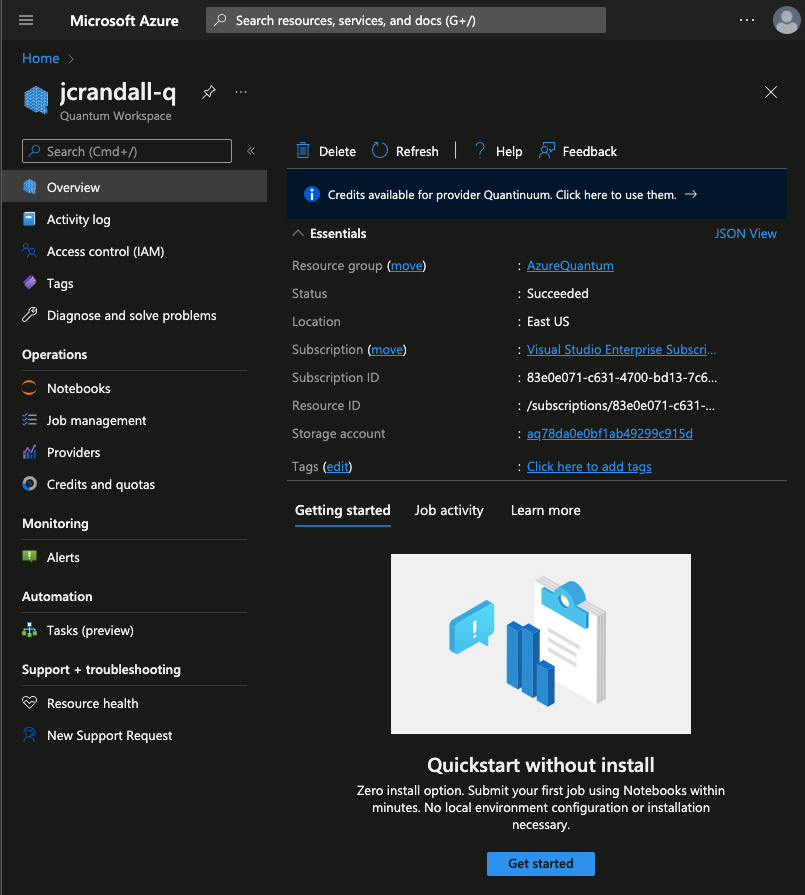
\includegraphics[width=5in]{paper/figs/quantumWorkspace.png}
            \caption{Quantum Workspace}
        \label{fig:quantumWorkspace}
    \end{figure}

     Code referenced in the paper is located in \href{https://github.com/jwcrandall/csci-6907-quantum-computing-project}{csci-6907-quantum-computing-project}.

\end{document}